\subsection{Recunstructed hyperons by CDS}
\begin{figure}[htbp]
  \centering
  \begin{tabular}{cc}
    \begin{minipage}{0.5\hsize}
      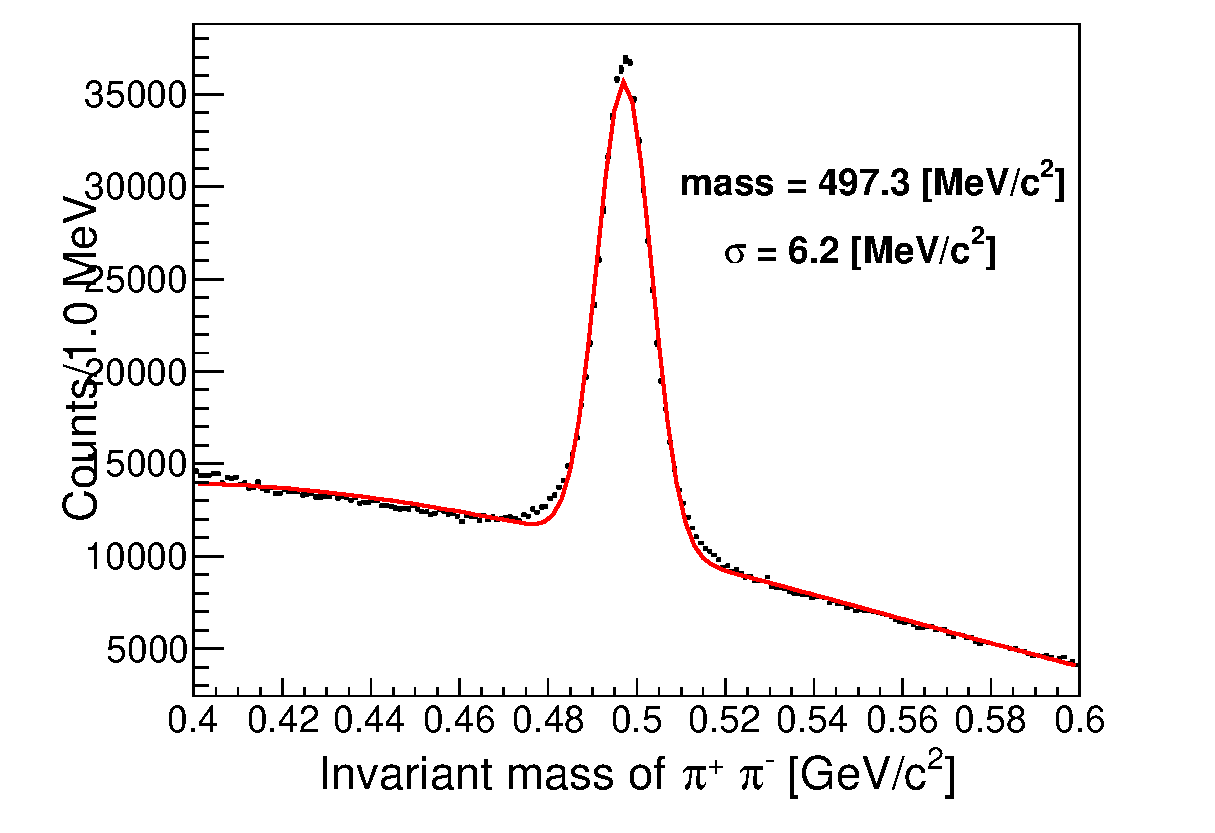
\includegraphics[width=5cm]{../pic/Run78/CDS/IM_pipi.eps}
    \end{minipage}
    \begin{minipage}{0.5\hsize}
      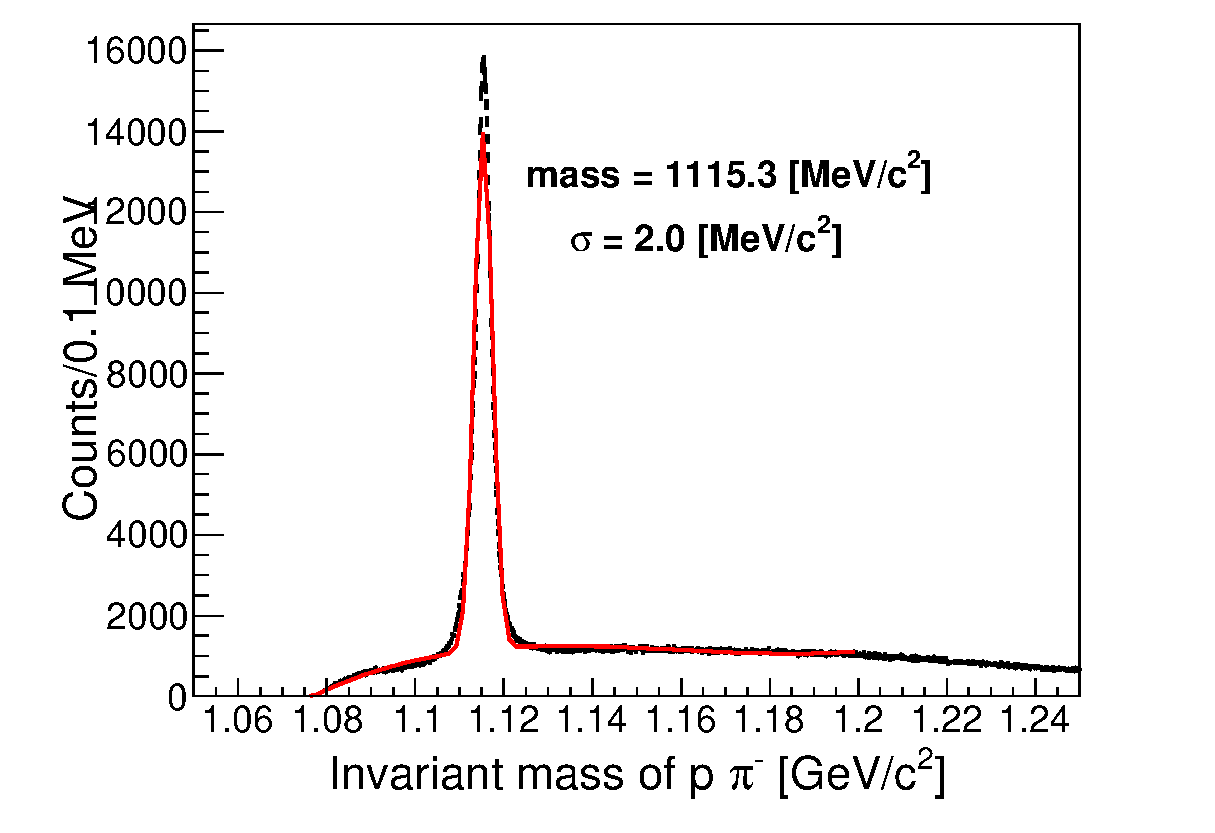
\includegraphics[width=5cm]{../pic/Run78/CDS/IM_ppim.eps}
    \end{minipage}
  \end{tabular}
  \caption{
    Left figure shows reconstructed $K^0$ from $\pi^+ \pi^-$ detected by the CDS.
    Right figure shows reconstructed $\Lambda$ from $p \pi^-$ detected by the CDS.
    Background function was evaluated by 5-th polynomial function.
  }
  \label{fig:CDS_IM}
\end{figure}

The $K^0$ and the $\Lambda$, well-known hyperons decay to $\pi^+$ $\pi^-$ and proton and $\pi^-$, respectively.
These decayed particles can be identified and momentum was reconstructed by the CDS as shown in Fig\ref{fig:CDS_IM}.

